% Section 6.6: Image Subtraction

\subsection{Image Subtraction}

The {\tt ip\_diffim} package implements the image subtraction
functionality in the {\tt IPSD}.  It was initially developed during
DC2, and is thus one of the more mature application packages in the
framework.  Much of the work during DC3a has gone into modifying the
code to use the new Applications Framework ({\tt afw})
pixel--processing interfaces, switching to a new third--party package
for the matrix math operations, a significant number of scripts to
unittest the Kernel creation, moving much of the pixel--processing
functionality from {\tt ip\_diffim} subroutines to apply() methods of
a class, implementation of more of the code in {\tt Python}, and
finally more a robust spatial modeling infrastructure.

\subsubsection{Implementation in Framework}

Two major {\tt afw} improvements facilitated the implementation of
{\tt ip\_diffim} for DC3a, both coming about due to the removal of
{\tt Vision Workbench} from the software stack.  The first was the
replacement of the {\tt VW} pixel access operations, while the second
was the adoption of the {\tt Eigen} package for linear algebra
operations.  

The {\tt afw} release version 3.1 included the first stable release of
the new pixel accessor and iterator functionality.  The entirety of
the {\tt ip\_diffim} C++ code base had to be updated to use this new
API.

The {\tt Eigen} matrix math library was adopted due to its speed and
templated design.  Compared to the {\tt VW} matrix math operations,
its considerably faster and cleaner to implement.  Using inversion of
a {\tt 500 x 500} matrix as a benchmark, VW could solve this problem
in 0.26 (using {\tt vw::math::least\_squares}) to 1.82 seconds (using
{\tt vw::math::pseudoinverse}).  In comparison, {\tt Eigen} has a
variety of methods to invert a matrix.  The fastest of these, Cholesky
decomposition (both with and without square root), takes 0.03 seconds
while LU decomposition takes 0.27 seconds.  This factor of 10 speedup
allows us to more robustly attempt to solve the matrix inverse, since
multiple attempts may be made using different options (e.g. attempt
Cholesky decomposition without square root; upon failure attempt
attempt Cholesky decomposition with square root, etc).


\subsubsection{Speed Ups}

Aside from the aforementioned linear algebra speed ups, as well as
caching improvements in the {\tt afw} convolution methods, we
implemented a specialization of convolution by delta function {\tt
Kernels}.  Since we are currently using delta functions as the basis
set for construction of our kernels, this sped up convolution by a
factor of {\bf XXX}.

\subsubsection{Algorithm Improvements}

The software went through a major redesign since DC2, in particular
based upon suggestions from management to make the package more
object--oriented.  This was accomplished using the {\tt
afw::detection::FootprintFunctor} class as a prototype and creating
several pixel--processing classes whose sole purpose is to iterate
over pixels and accumulate statistics.  The most noteworthy of these
is the {\tt PsfMatchingFunctor} class, which builds a single Psf
matching Kernel given 2 input images (the template and science image).
Finally, the vast majority of the code structure was implemented in
{\tt Python}.

The major improvement in the {\tt ip\_diffim} package over DC2 was in
designing an infrastructure for the spatial modeling of the Kernel.
The {\tt SpatialCell} class divides the image up into a grid, and
attempts to build a single Kernel model for each Cell by choosing the
brightest object to build a Kernel around (using a {\tt
PsfMatchingFunctor}).  If that model turns out to be inadequate
(i.e. the resulting difference image is noisier than is acceptable),
another object is used in the modeling.  This process is repeated
until a good Kernel is found, or all objects are deemed to be
inadequate, in which case the Cell is considered ``empty''.  In this
way we generate an even grid of constraints of the Kernel model across
the image, which will facilitate the creation of the spatial Kernel
model.  The spatial fitting is now integrated closely with the {\tt
SpatialCell} class, iterating over all Cells and using their
respective models as constraints on the Kernel.

The input variance is now accepted as an argument to the Psf matching
step.  An initial estimate of the variance in the final difference
image, used in the denominator of the weighted $\chi^2$ calculation
that leads to the Kernel solution, is just a basic image subtraction
without convolution.  In cases where the image being convolved has
negligible variance, this is a good estimate.  However, if the
convolution happens to an image with low signal--to--noise, this
estimate will be poor.  In this case, the input variance may be
recalculated using the difference of the science image and template
convolved with the first Kernel solution.  This variance can be used
in a second iteration of Kernel creation.  The variance and thus the
Kernel are shown to converge after one iteration of this process, in
the case where the image being convolved is single--depth.

Additional minor improvements in {\tt ip\_diffim} include a means of
growing the {\tt Footprints} around sources by a fraction of the
Kernel size.  This is to provide enough unconvolved pixels to
constrain each of the Kernel elements.  The ratio at which the Kernel
sum converges appears to be at a minimum a grow by a factor of 1.5,
although a factor of 2.0 was used for DC3a to be conservative.  In
addition, we have vastly decreased the number of eigenKernels being
used in the spatial model.  Runs using 25 and 10 eigenKernels were
performed; we predict that as we understand the Kernel creation more
we should have to use no more than 5 eigenKernels in the spatial
model.  This will speed up processing considerably.

\subsubsection{Results for CFHT}

The single--source Kernels are working optimally, in the sense that
the residuals in the difference image appear to be at the noise limit.
To be explicit, after creation of the difference image we divide the
image pixels by the square root of the variance pixels.  This is the
$\chi$ value, and the distribution of this across the difference image
should have a mean of 0.0 and root--mean--square deviation of 1.0.
This is accomplished in practice for the vast majority of sources.
However, for very bright stars (peak counts near 40,000 or above) the
difference image frequently has too large of residuals.  These single
Kernels are sigma clipped from the spatial Kernel fit.
Figure~\ref{fig:diffim} illustrates an acceptable difference image
({\it top row}) and one that fails ({\it bottom row}).  

\begin{figure*}[htp]
\centering
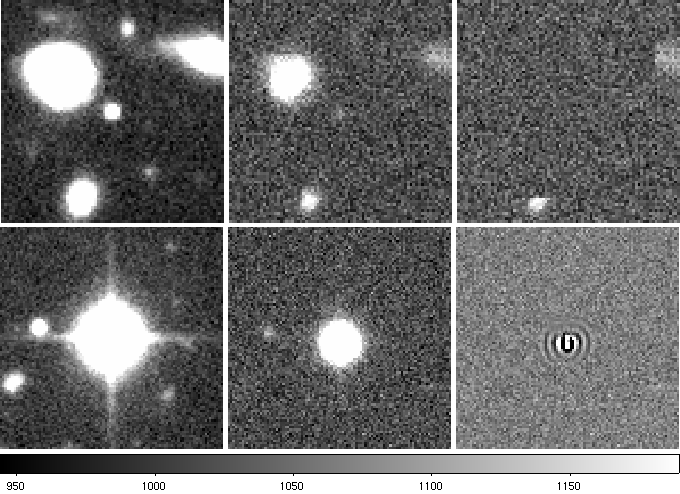
\includegraphics[]{images/diffim.png}
\caption[Example difference images.]
{ Each row shows a set of difference images, displayed left--to--right
as the template image, the science image, and the resulting difference
image.  For the top row, the difference image is clean, with only
objects at the border left unsubtracted (these pixels are masked due
to the convolution).  Even objects off--center subtract cleanly, and
some in fact are split in half.  The bottom row shows a set of images
where the object did not subtract cleanly.  These effects were found
in the brightest objects; we suspect this is partially due to the
complicated shape of the star in the template image, and emphasizes
that we need to be careful when constructing our image subtraction
templates in future data challenges.  }
\label{fig:diffim}
\end{figure*}

We have been in contact with the CFHT team regarding aspects of their
data that might make the shapes of bright stars different than the
shapes of the fainter stars.  CFHT apply no linearity corrections to
their data.  However, they have done tests using multiple exposure
times on a given star field and find that star fluxes are not affected
at the level of a few millimagnitudes (Astier 2009, private
communication).  This suggests that non--linearity is not a
significant issue.  More likely is that the shapes of the bright stars
in the template images we are differencing against are complicated.
Of particular note are the relative shapes of the cores of the
objects, and the relative shapes of the wings of the objects.  If
these two regimes require a different PSF--matching Kernel, the entire
process will return a solution that is not optimal for either.  We
suspect that the shapes of the brightest stars have changed during the
coaddition process, which uses a median combine
algorithm\footnote{This is seen in the template Fits header as {\tt
COMBINET= 'MEDIAN ' / COMBINE\_TYPE config parameter for SWarp}.}.  It
is likely that pixels at the centers of the bright stars contribute to
the stack with a strong dependence on seeing, making these poor
objects for Psf matching.

We note that we were unable to use the simulated images (both SimDeep
and SimWide) for the image subtraction portion of {\tt IPSD} since the
template images are severely undersampled (0.1'' seeing with 0.3''
pixels).

\subsubsection{Future Work}

Further investigation of the convolution vs. deconvolution issue is
certainly warranted.  Using single--depth images from the {\tt
SimDeep} dataset, we have determined that the derived Kernels are far
noisier than expected even when the process is known to be a
(smoothing) convolution since we have controlled all the variables in
creating the images -- we know both the seeings of the images and that
the Psfs should be similarly different across the full dynamic range
in brightness.  This is puzzling, since unit tests that apply both a
known smearing Kernel and the addition of noise to the image recover
the smearing Kernel around single sources and as the mean Kernel
across all sources, with small values in the eigenKernels.  We are
consulting with Paul Price who has written the equivalent of {\tt
ip\_diffim} for the Pan-STARRS Image Processing Pipeline.  For
reference, he is currently using an Alard--Lupton (sum of 3 Gaussians)
basis having written and decided not to use a delta function basis.
However, Pan-STARRS has not implemented a Principal Component Analysis
of the derived single Kernels, which should address many of the
perceived weaknesses of the delta function basis set (not generally
smooth, especially at the edges; not generally trending to zero at the
edges).  Nevertheless post--DC3a we will be implementing a sum of
Gaussians basis set similar to Alard--Lupton for further testing.

We will also address the scaling of the Kernel sizes with the full
width at half maximum (FWHM) of the input images.  They should be
large enough to have enough power where the Psfs are most different,
but not too large to slow down processing.

Finally the {\tt SpatialCell} functionality was initially written for
fitting of the {\tt ip\_diffim} convolution Kernel.  However, it was
subsequently rewritten in a more advanced form for modeling of the
spatially varying Point Spread Function.  A task post--DC3a is to
update {\tt ip\_diffim} to use this newer SpatialCell functionality,
essentially merging the {\tt ip\_diffim} Kernel and Psf fitting tasks
with a common toolset.
